\section{Vypracování}

Pro vypraccování semestrální práce byly zvoleny parametry dle zadání.
Jedinými vlastními parametry jsou hladina významnosti \( \alpha = 0.5\) a \textit{tail}, nutné jako parametry funkce \textit{ttest2}.
Hodnota \( \alpha \) byla zvolená jakožto výchozí hodnota dle dokumentace programu MATLAB.
Pro alternativní hypotézu (\textit{tail}), byla zvolená hodnota \textit{right}, dle dokumentace \enquote{mean of X is greater than mean of Y (right-tailed test)}.

Při testování významnosti nulové hypotézy je p-hodnota pravděpodobnost získání výsledků testu takových, jako jsou skutečně pozorované výsledky, za předpokladu, že je nulová hypotéza správná.
Je~tedy hladinou, od které je nulová hypotéza zamítána.

\subsection{Výsledky hypotéz}

Tabulky~\ref{table:table1} a~\ref{table:table2} zobrazují zamítnutí, či potvrzení hypotézy rovnosti středních hodnot, popřípadě toho, že střední hodnota levého souboru je větší než středního hodnota pravého souboru vzorků.
Jestliže je v~tabulce hodnota jedna, pak je hypotéza zamítnuta a \textit{vice versa}.

\begin{table}[htb]
    \centering

    \begin{tabular}{rccc}
        \toprule

        Počet vzorků    & (A', B')  & (A', C') & (B', C')   \\ \midrule
           5            & 0         & 0        & 1          \\
          10            & 0         & 0        & 0          \\
          20            & 0         & 0        & 0          \\
          50            & 0         & 0        & 0          \\
         100            & 0         & 0        & 0          \\
         200            & 0         & 0        & 0          \\
         500            & 0         & 0        & 0          \\
        1000            & 0         & 0        & 0          \\
        2000            & 0         & 0        & 0          \\

        \bottomrule
    \end{tabular}

    \caption{Výsledné hypotézy jednostranného dvouvýběrového t-testu.}
    \label{table:table1}
\end{table}
\FloatBarrier

V tabulce~\ref{table:table1} si můžeme všimnout \textit{outliera} hned v první řádce.
Hodnota 1 u souborů B a C říká, že hypotéza \enquote{střední hodnota souboru B je větší než střední hodnota souboru C} je zamítnuta.
Zbytek tabulky však odkrývá opačný trend.
Výsledek lze tedy klást za vinu nedostatečnému počtu vzorků, zvláště vezmeme-li v úvahu, že střední hodnota souboru C má být desetkrát větší než střední hodnota souboru B.

\begin{table}[htb]
    \centering

    \begin{tabular}{rccc}
        \toprule

        Počet vzorků    & (A', B')  & (A', C') & (B', C')   \\ \midrule
           5            & 1         & 0        & 0          \\
          10            & 0         & 0        & 0          \\
          20            & 0         & 1        & 0          \\
          50            & 0         & 1        & 0          \\
         100            & 0         & 0        & 0          \\
         200            & 0         & 1        & 1          \\
         500            & 0         & 1        & 1          \\
        1000            & 0         & 1        & 1          \\
        2000            & 1         & 1        & 1          \\

        \bottomrule
    \end{tabular}

    \caption{Výsledné hypotézy oboustranného dvouvýběrového t-testu.}
    \label{table:table2}
\end{table}
\FloatBarrier

O výsledcích v druhé tabulce lze uvažovat podobně jako v případě tabulky první.
Nesrovnalosti oproti očekáváním jsou jistě způsobeny nedostatečným počtem vzorků.

\subsection{p-hodnoty}

\begin{figure}[htb]
    \centering
    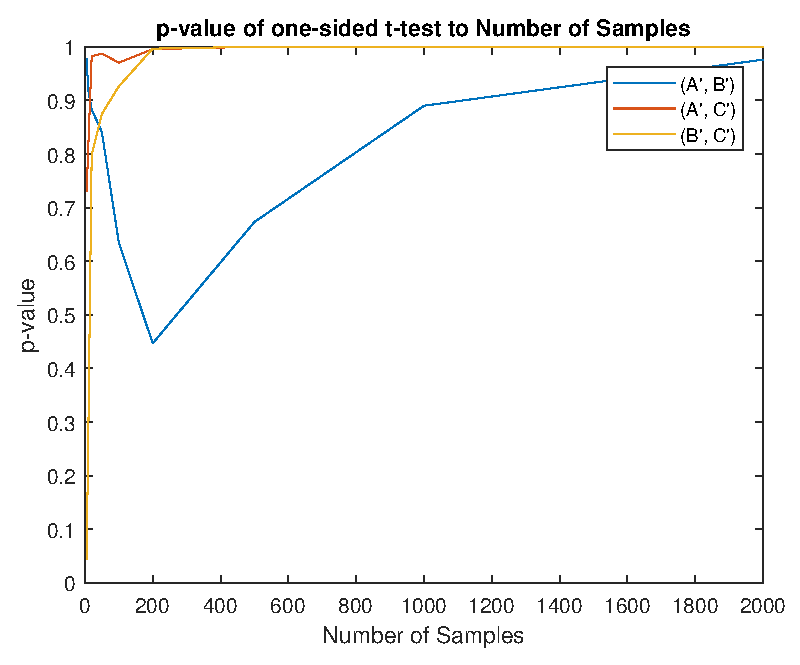
\includegraphics[width=0.55\textwidth]{graphs/fig1.eps}
    \caption{Závislost p-hodnoty jednostranného dvouvýběrového t-testu na velikosti souboru měření.}
    \label{fig:test1}
\end{figure}
\FloatBarrier

\begin{figure}[htb]
    \centering
    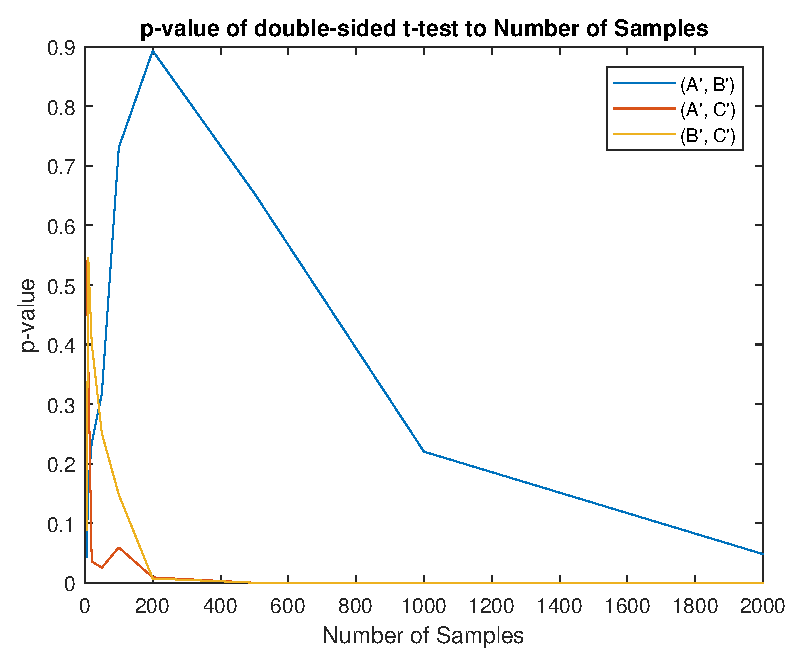
\includegraphics[width=0.55\textwidth]{graphs/fig2.eps}
    \caption{Závislost p-hodnoty oboustranného dvouvýběrového t-testu na velikosti souboru měření.}
    \label{fig:test2}
\end{figure}
\FloatBarrier

\section{Závěr}

Výsledky experimentů nejsou nijak překvapivé.
Čím měně je k dispozici vzorků, tím méně se dá spolehnout na pravdivost výsledků testů.

Na grafech si lze povšimnout vývoje p-hodnot (hodnota od které je nulová hypotéza zamítána).
Ta je v případě hypotézy rovnosti středních hodnot klesající, v případě jejich \enquote{pravé} nerovnosti je rostoucí.
